\chapter{Determination of the relevant scales}

We base our study on the center of galaxy clusters at low redshift so it is necessary to study the scales that we will be relevant for our studies. In order to calculate the range of scales that we will probe in the observational procedures on chapter 4 we will do two separate experiments. The first one is the study of the amount of objects that we would expect to be lensed near the cluster centres by using a very extensive catalogue of galaxies. The second one consists on doing the mass modelling of the cluster for its stellar and dark matter content to see on which scale stars are the main component of the enclosed mass that lenses background objects.

For our first experiment, we make use of the COSMOS2015 catalogue (Laigle et. al. \citeyear{Reference21}) which contains half a million objects in a range of $1<z<6$. Ricardo Herbonnet matched the CFHT data to this catalogue so we use his matched data which contains a total of 133,348 galaxies in the 2 degree COSMOS field. We count the amount of galaxies for different magnitudes in redshift bins of $0.2z$ for the R filter. These numbers represents the expected number of galaxies in the background of the lens objects of our sample as seen in figure []. 

\begin{figure}[H]
\centering
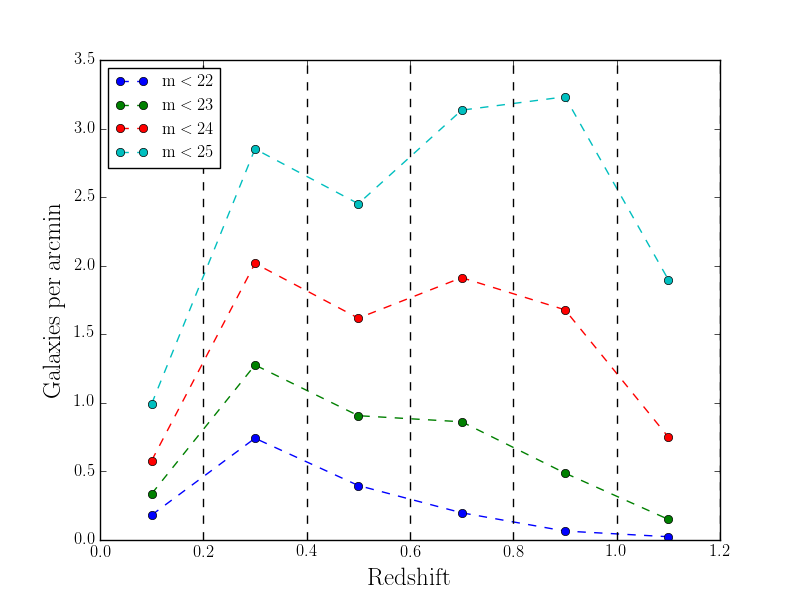
\includegraphics[width=12cm]{images/galaxies_per_arcmin.png}
\caption[Galaxies per arcmin]{Galaxies per arcmin$^2$ in redshift bins of $0.2z$. }
\end{figure}

Around z=0.3 we find the peak of the number of galaxies so it is the redshift that is most likely to contain galaxies that could be seen in our data. For the deepness of our data of around 23 mag (as discussed in the next chapter) we then expect some background galaxies for which we can measure the Einstein ring, although the number is rather small. 

CFHT can see objects as deep as m=23 but Hubble Space Telescope could see objects as deep as m=25 so it should be able to see a lot more objects that have been lensed.

For the second experiment, we will check the scale of dominance of dark matter by using the NFW dark matter halo profile (since galaxy clusters are known to be dominated by their dark matter content) and the de Vaucouleurs profile, (1948) to compare the contribution of stars in comparisson to dark matter, this will allow us to see in which scales the DM mass becomes dominant thus making it more difficult to constrain the stellar content of the bright galaxy.

The plot of the enclosed mass shows what radial scale we need to probe. One way could be through dynamics, another could be through gravitational lensing. If we take different IMFs, how sensitive is the matter content to the choice of IMF?. Smaller the dark matter contribution, the smaller the overall error you make since light is easier to constraint and thus the IMF. Strong lensing measures exactly the enclosed mass so we need to know how much of its contribution we need to subtract, the less we have to subtract, the better for the determination of the IMF. If the effect of the IMF is very subtle in the mass vs radius plot, then we would need to know the dark matter distribution very well, but if the effect of the IMF is not very subtle, the less you need to know about the dark matter distribution. A recent study of a BCG mentions the relevance of this spatial scale, at very small radii stars dominate the lensing mass, so that lensing provides a direct probe of the stellar mass-to-light ratio, with only small corrections needed for dark matter (Russell Smith and John R. Lucey \citeyear{Reference7}) 

That's why the IMF is relevant, because it allows to see how much it moves up and down. If you look at a galaxy, why is it not possible to get the mass to light ratio? This is because the dark matter is more diluted than stellar light so the mass follows light behaviour is not valid and a well understood theory of the dark matter halos has to be taken into account, NFW (Navarro, Frenk \& White, \citeyear{Reference17}) provided a very consistent model for dark matter halos using N-body simulations so we can relate the lensing of the halos given this NFW density profile and putting special attention in the spacial scales on which the dark matter is relevant and where it starts to be the dominant contribution of the system and thus the lensing.

From Lokas\& Mamon \citeyear{Reference14}, for constant mass-to-light-ratio we have $\Sigma_{\text{M}}(R)= \Upsilon I(R)$ where $I(R)\approx 10^{7}$ was found by fitting the surface brightness with \texttt{GALFIT}.

The mass to light ratio for a Salpeter IMF is $\Upsilon\approx 4$

Let's take the case of ABELL1068, it's magnitude in U is 21.94, in I is 18.46, in g is 20.09, in r is 19.5, also $\text{M}_{200}=4.3\times 10^{14}\text{M}_{\odot}$ (van der Burg et. al 2015)

The bolometric luminosity of Abell1068 is $10^{44}$erg/s that in solar luminosities is $1.9\times 10^{12} L_{\odot}$, this gives an effective brightness of $0.962\times 10^{7}\text{M}_{\odot}/\text{kpc}^2$.

In the case of the ABELL1068 cluster, our estimation yields a concentration parameter of 4.46 (using figure of the concentration parameter in the previous chapter).

The critical density would be: $2\times 10^{-26}kg/m^{3}$ in SI units so in $\text{M}_{\odot}/\text{pc}^{3}$ it is $2.9\times 10^{-7}$

the Hubble parameter at z=0.138 is H(z)=85.6

The characteristic radius is given by $r_{1/2}=1.34R_{e}$

For the stellar content of the cluster we can use de Vaucouleurs law for the surface brightness distribution in giant elliptical galaxies which is:

\begin{equation}
I(R)=I_{e}e^{-b\left[\left(R/R_{e}\right)^{1/4}-1\right]}
\end{equation}

where $b=7.67$ and $I_{e}$ is the effective brightness which is basically the brightness at the effective radius $R_{e}$

Hence we have the surface mass density for both the stellar content and the NFW profile, as shown in figure [].

\begin{figure}[H]
\centering
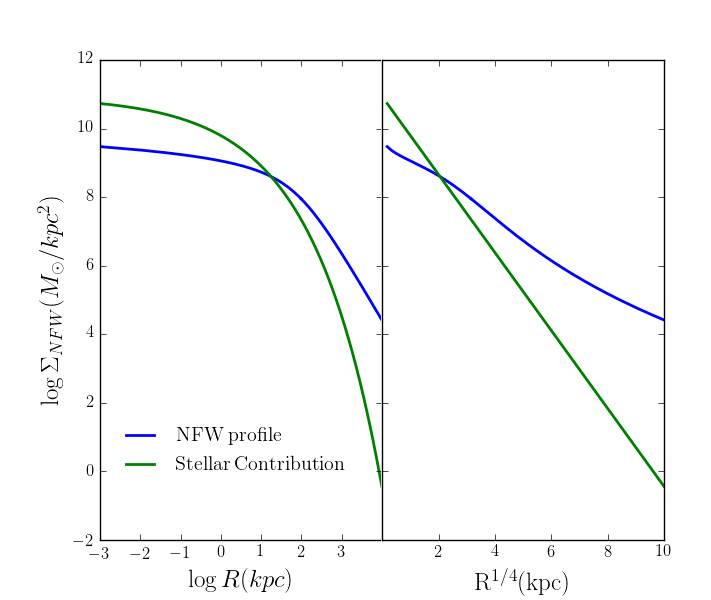
\includegraphics[width=12cm]{images/Surface_mass_density_log.png}
\caption[Surface mass density profiles]{Surface mass density profiles in logarithmic and $R^{1/4}$ scale for the NFW profile and the stellar component.}
\end{figure}

And we can recover our luminosity by integrating the surface brightness profile accordingly:

\begin{equation}
L=\int_{0}^{R}2\pi RI(R)dR
\end{equation}

The integration gives a value that is comparable to the one found using Faber-Jackson relation: $L=\Upsilon\times\sigma^{4}\approx 1.2\times 10^{12}\text{M}_{\odot}$

The value found for the mass in light is $\text{M}_{\star}=2.582\times 10^{11}\text{M}_{\odot}$ and the mass given by the NFW profile is $\text{M}_{\text{NFW}}=6.557\times 10^{11}\text{M}_{\odot}$.

The enclosed mass profile for dark matter and stellar matter for different IMFs (Chabrier, Kroupa, Salpeter) is shown in figure [].

\begin{figure}[H]
\centering
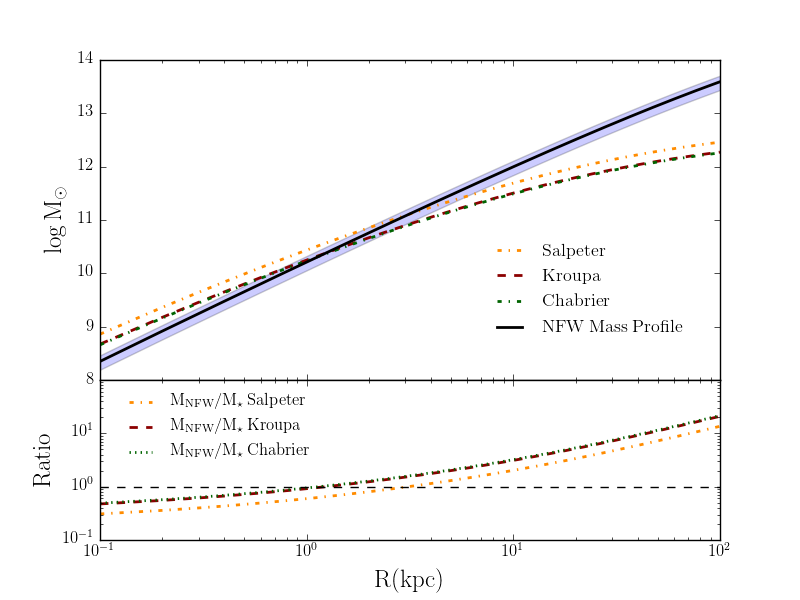
\includegraphics[width=12cm]{images/DM_fraction_all_IMFs.png}
\caption[Enclosed mass and DM to stellar mass ratio]{Enclosed mass and DM to stellar mass ratio}
\end{figure}

This result suggests that it is very difficult to make a detailed study if the the stellar content of the BCG because the gravitational lensing associated to it would be mostly caused by the dark matter component at almost all scales. The stellar content is only dominant in the innermost region, quite far from the Einstein radius which is constrained by the total enclosed mass (dark matter and stars).

It is then useful to study cases in which the lens system is an elliptical galaxy following its own dark matter halo and not inside the potential well of a cluster in the case of the BCG. As calculated by Sonnenfeld et. al. \citeyear{Reference15}, the encounter of the enclosed mass profiles for DM and stars for the system SDSSJ0946+1006, also known as the "Jackpot" is $~3\text{kp}$ as seen in figure [] which is a larger radius than the one calculated for a BCG immerse in the halo of a low redshift cluster of around $~1.5\text{kp}$.  

The values for this galaxy are: 

z=0.222, c=10**0.9, $delta_c=25644.5=7.9428$, $M_{star}=5.5\times 10**11 M_{\odot}$

\begin{figure}[H]
\centering
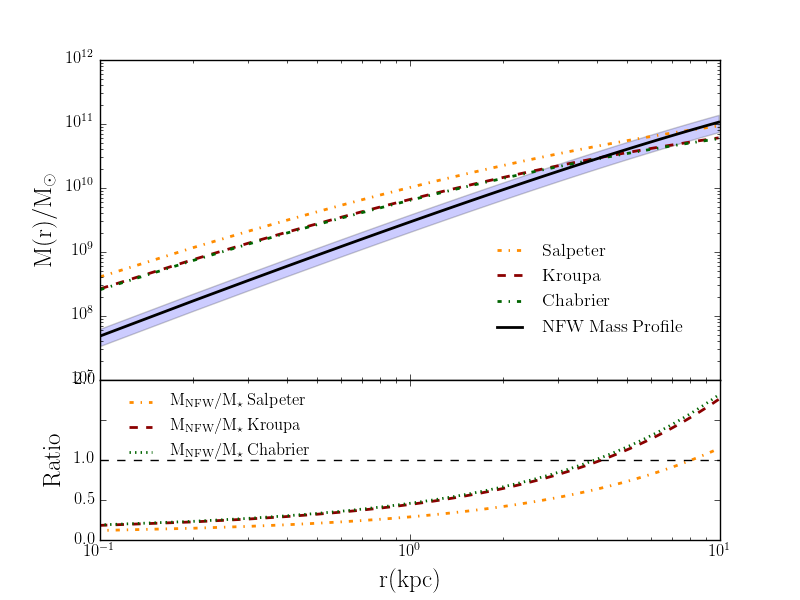
\includegraphics[width=12cm]{images/DM_fraction_all_IMFs_galaxy.png}
\caption[DM and Stellar mass profiles for a massive early type galaxy.]{Mass profile for dark matter and stellar content for the lens system SDSSJ0946+1006.}
\end{figure}

Now, we are interested in having an accurate estimate of the Einstein radius to constraint the model, so we make different analysis on the radial dependence on the lensing properties such as shear, reduced shear and magnification.

The shear dependence on radius is shown in figure [].

\begin{figure}[H]
\centering
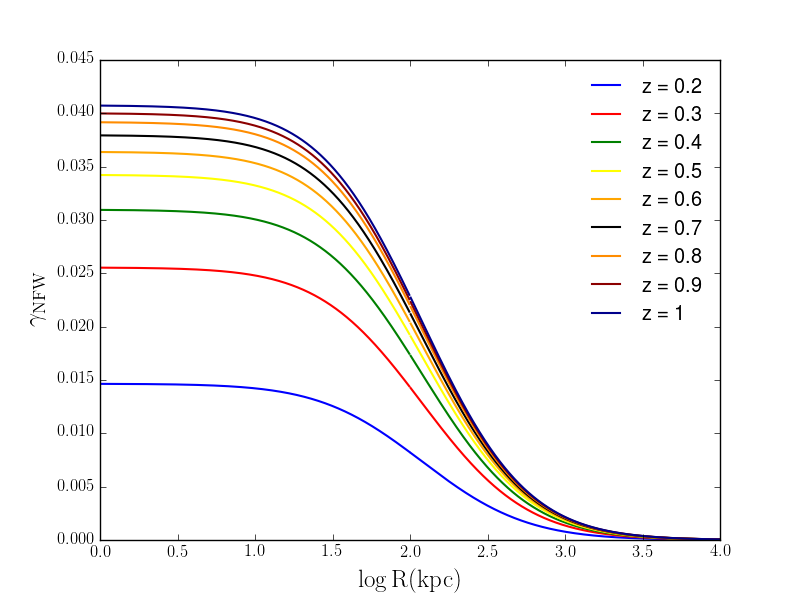
\includegraphics[width=12cm]{images/Shear_vs_rad.png}
\caption[Shear dependence on radius]{Shear dependence on radius for different redshift of the background galaxies}
\end{figure}

Figure [] shows the magnification.

\begin{figure}[H]
\centering
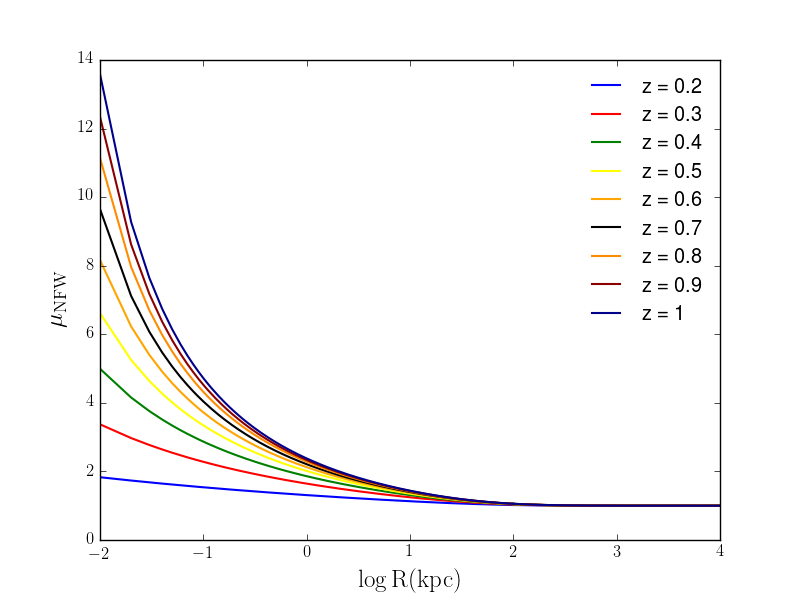
\includegraphics[width=12cm]{images/Magnification.png}
\caption[Magnification radial profile]{Magnification radial profile for various redshifts}
\end{figure}

The reduced shear is given by:

\begin{equation}
g=\frac{\gamma}{1-\kappa}
\end{equation}

The reduced shear for background objects at different redshifts is shown in figure []. 

\begin{figure}[H]
\centering
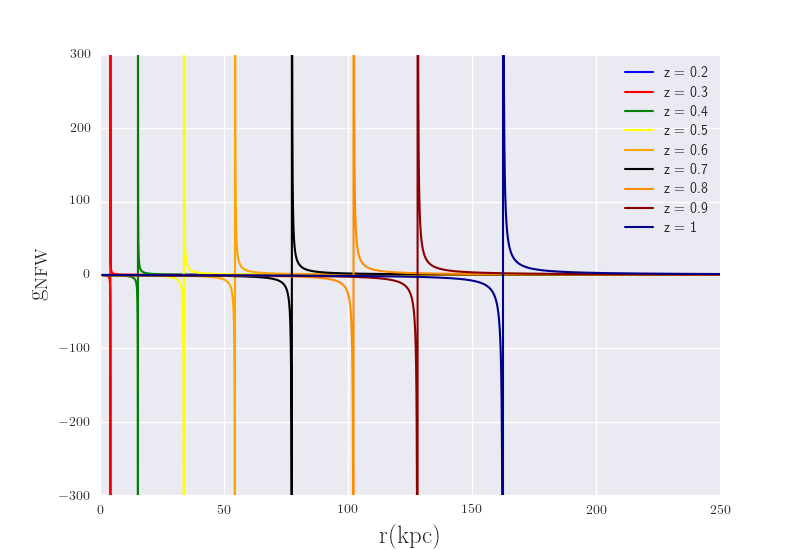
\includegraphics[width=12cm]{images/Reduced_Shear.png}
\caption[Reduced shear radial]{Reduced shear radial profile for different redshifts.}
\end{figure}

so we get the Einstein ring where $\mu$ is infinite or when g is 1 ($\kappa=1/2$)
